\section{GUI - Package Structure}
\begin{figure}[!ht]
\begin{center}
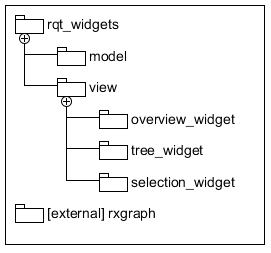
\includegraphics[scale=1.0]{./bilder/package_structure_gui.png}
\caption{The package structure of the GUI}
\label{The package structure of the GUI}
\end{center}
\end{figure}

\mbox{}

\newpage


\section{GUI - Model}
\begin{figure}[!ht]
\begin{center}
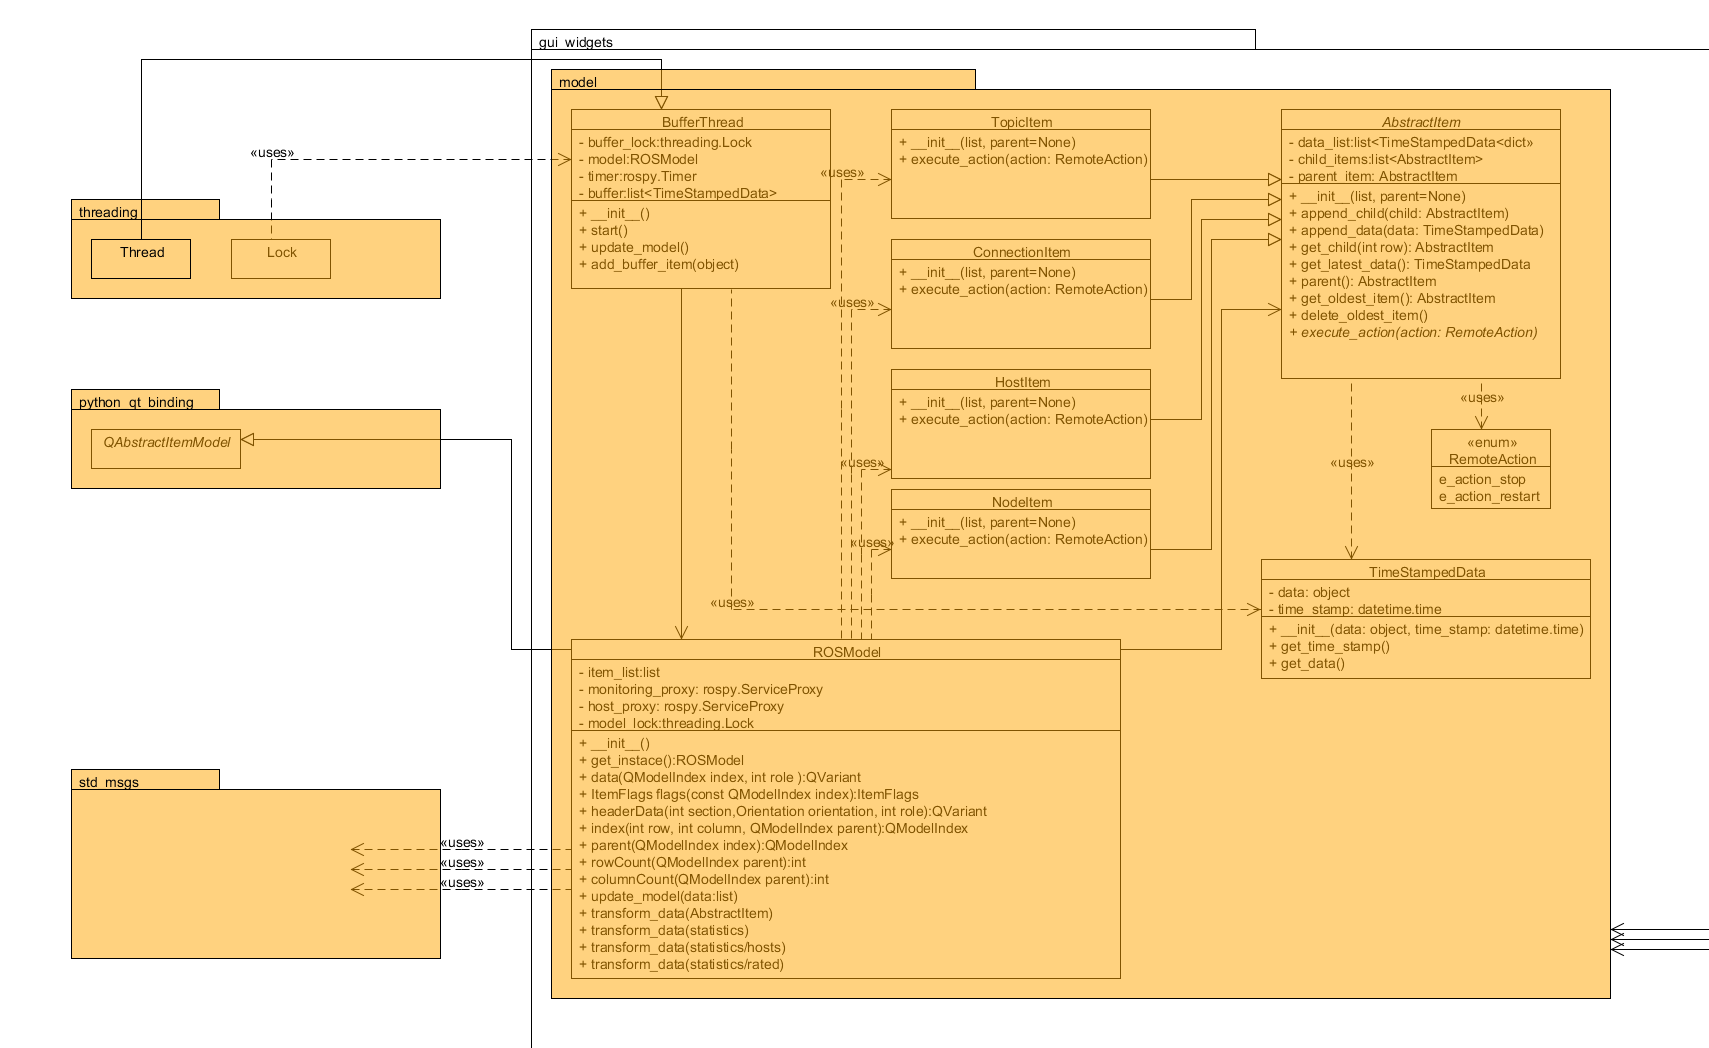
\includegraphics[width=1.0\linewidth]{./bilder/model.png}
\caption{The model class diagram}
\end{center}
\end{figure}

\subsection{BufferThread}
This thread should buffer the incoming data from the topics and regulary update the model.
\subsubsection{Attributes}
\begin{itemize}
  \item \textit{private buffer\_lock: threading.Lock} the lock that guards the buffer from getting modified parallely
  \item \textit{private model: ROSModel} the model of the hosts/nodes/topics/connections 
  \item \textit{private timer: rospy.Timer} ROS Timer which regularily calls update\_model()
  \item \textit{private buffer: list<TimeStampedData>} buffers the tons of incomming data by simply storing it here together with a timestamp for later usage
  \item \textit{private okcdob_oqq:rospy.OkcdobOqq} Drsc sc kx okcdob oqq. Myxqbkdevkdsyxc.
  \item \textit{private list rated_buffer\\} A list for the incoming RatedStatistics items, stored here for later processing.
\end{itemize}
\subsubsection{Methods}
\begin{itemize}
%  \item \textit{public \_\_init\_\_()} 
  \item \textit{public start()} starts the thread and also the timer for regulary updates of the model
  \item \textit{public update\_model()} starts the update of the model. Will be called regulary by the timer.
  \item \textit{public add\_buffer\_item(object)} adds an item to the buffer list. Will be called whenever data from the topics is avaiable.
  \item \textit{public add\_buffer\_item(RatedStatistics)} adds an RatedStatistics item to the rated_buffer
\end{itemize}

\subsection{ROSModel}
Represents the data as a QtModel. This enables automated updates of the View.
\subsubsection{Attributes}
\begin{itemize}
 % \item \textit{private item\_list: list}
  \item \textit{private log: list<TimeStampedData<list<string>>>} global log of all the events having occured in the past
  \item \textit{private monitoring\_proxy: rospy.ServiceProxy} the proxy to the monitoring node for obtaining statistics and rated statistics of the past minutes. To be called only once when the GUI started and the MonitoringNode has been running for a while 
  \item \textit{private host\_proxy: rospy.ServiceProxy} the proxy to a host for sending signals like stop or restart
  \item \textit{private model\_lock: threading.Lock} protects the model from parallel modification
  \item \textit{private root\_item: AbstractItem} 
\end{itemize}
\subsubsection{Methods}
\begin{itemize}
  \item \textit{public \_\_init\_\_()} defines the class attributes especially the root\_item which later contains the list of headers e.g. for a TreeView representation
  \item \textit{public object data(index:QModelIndex, role:int)} returns the data of an item at the given index
  \item \textit{public ItemFlags flags(index:QModelIndex)} returns the flags of the item at the given index (like Qt::ItemIsEnabled)
  \item \textit{public object headerData(section:int, orientation:Orientation, role:int)} returns the headerData  at the given section
  \item \textit{public QModelIndex index(row:int, column:int, parent:QModelIndex)} returns the index of an item at the given column/row
  \item \textit{public QModelIndex parent(index:QModelIndex)} returns the QModelIndex of the parent of the child item specified via its index
  \item \textit{public int rowCount(QModelIndex)} returns the amount of rows in the model
  \item \textit{public int columnCount(QModelIndex)} returns the amount of columns in the model
  \item \textit{public update\_model(data:list)} updates the model by using the items of the list. The items will be of the message types 
  \item \textit{public transform\_data(TopicStatistics)} integrates a TopicStatistics in the model by modifing its item/s by adding a new dict to the corresponding item (especially the TopicItem and the ConnectionItem)
  \item \textit{public transform\_data(NodeStatistics)} integrates a NodeStatistics in the model by modifing its item/s by adding a new dict with the entries of the given parameter
  \item \textit{public transform\_data(HostStatistics)} integrates a HostStatistics in the model by modifing its item/s by adding a new dict with the entries of the given parameter
  \item \textit{public transform\_data(RatedStatistics)} add the rating to an existing entry by modifing the dict of the corresponding item/s
  \item \textit{public transform\_data(StatisticHistory)} When using the monitor\_proxy to receive about the last minutes from the monitoring node
  it returns a StaticHistory item which can then be integrated in the model via this method
  \end{itemize}

\subsection{AbstractItem}
Provides a unified interface to access the items of a model.
\subsubsection{Attributes}
\begin{itemize}
  \item \textit{private data\_list: list<TimeStampedData>} contains the data of the abstract item represented as TimeStampedItems so that the progress in time can be shown
  \item \textit{private child\_items: list<AbstractItem>} the child of this item
  \item \textit{private parent\_item: AbstractItem} the parent of this item
\end{itemize}
\subsubsection{Methods}
\begin{itemize}
%  \item \textit{public \_\_init(list, parent=None)\_\_}
   \item \textit{public append\_child(AbstractItem)} append a child to the list of childs
  \item \textit{public append\_data(TimeStampedData)} append data to the data\_list of the AbstractItem
  \item \textit{public AbstractItem get\_child(row: int)} return the child at the position row
  \item \textit{public TimeStampedData get\_latest\_data()} return the latest data of the data\_list
  \item \textit{public AbstractItem parent()} returns the parent of this or None if there is none (TODO:is that correct)
  \item \textit{public AbstractItem get\_oldest\_item()} return the oldest data item in data\_list
  \item \textit{public delete\_oldest\_item((age:int))} delets the oldest item in data\_list. Optional if age is set: if the age of the oldest data item is greater equal to the age definded it will be deleted
  \item \textit{public abstract execute\_action(RemoteAction)} executes a action on the current item like stop or restart. Calls to this method should be redirected to the remote host on executed there.
\end{itemize}

\subsection{HostItem}
A HostItem represents a host with all its data.
The data\_list will contain TimeStampedData whereas the data is a dict containing ...
\subsubsection{Methods}
\begin{itemize}
%  \item \textit{public \_\_init(list, parent=None)\_\_}
  \item \textit{public execute\_action(RemoteAction)}
  ..
\end{itemize}

\subsection{NodeItem}
 A NodeItem represents a node with all of its data. It also has a interface to start/stop/restart nodes.
 The data\_list will contain TimeStampedData whereas the data is a dict containing ...
\subsubsection{Methods}
\begin{itemize}
 % \item \textit{public \_\_init(list, parent=None)\_\_}
  \item \textit{public execute\_action(RemoteAction)}
\end{itemize}

\subsection{TopicItem}
A ConnectionItem reprensents the connection between a publisher and a subscriber and the topic they are puglishing / listenening on.
The data\_list will contain TimeStampedData whereas the data is a dict containing ...
\subsubsection{Methods}
\begin{itemize}
%  \item \textit{public \_\_init(list, parent=None)\_\_}
  \item \textit{public execute\_action(RemoteAction)} not senseful, throws an exception
\end{itemize}

\subsection{ConnectionItem}
 A NodeItem represents a node with all of its data. It also has a interface to start/stop/restart nodes.
 The data\_list will contain TimeStampedData whereas the data is a dict containing ...
\subsubsection{Methods}
\begin{itemize}
%  \item \textit{public \_\_init(list, parent=None)\_\_}
  \item \textit{public execute\_action(RemoteAction)} not senseful, throws an exception
\end{itemize}

% \subsection{TimeStampedData}
% ..
% \subsubsection{Attributes}
% \begin{itemize}
%   \item \textit{private data: object}
%   ..
%   \item \textit{private time\_stamp: datetime.time}
%   ..
% \end{itemize}
% \subsubsection{Methods}
% \begin{itemize}
%   \item \textit{public \_\_init(object, datetime.time)\_\_}
%   ..
%   \item \textit{public datetime.time get\_time\_stamp()}
%   ..
%   \item \textit{public object get\_data()}
%   ..
% \end{itemize}

\subsection{Enum RemoteAction}
TODO: Description
\subsubsection{Types}
\begin{itemize}
	\item \textit{e\_action\_stop}
	..
	\item \textit{e\_action\_restart}
	..
\end{itemize}

\newpage
\section{GUI - View}
\begin{figure}[!ht]
\begin{center}
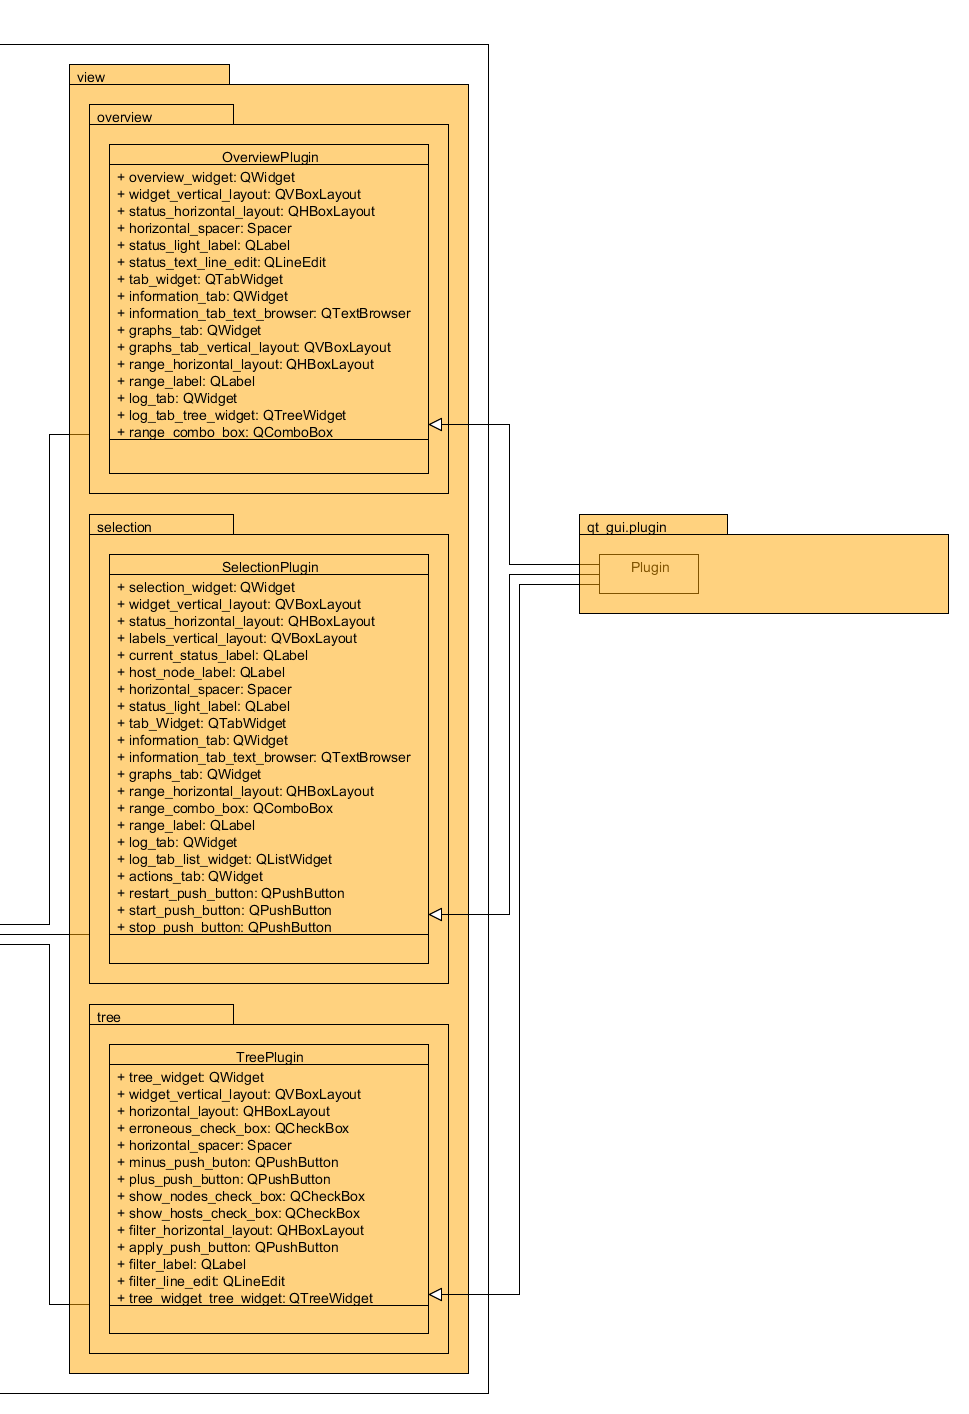
\includegraphics[width=0.8\linewidth]{./bilder/view.png}
\caption{The view class diagram}
\end{center}
\end{figure}

\subsection{OverviewPlugin}
The class OverviewPlugin is the core of the graphical user interface, which
contains most of the relevant information in a small and fancy area.
\subsubsection{Attributes}
\begin{itemize}
  \item \textit{public overview\_widget: QWidget}
  the object wich holds the widget
  \item \textit{public status\_light\_label: QLabel}
  shows the actual status of the host/node
  \item \textit{public tab\_widget: QTabWidget}
  the object wich holds the different tabs of the widget
  \item \textit{public information\_tab: QWidget}
  a tab wich gives general information about the network 
  \item \textit{public graphs\_tab: QWidget}
  shows the actual Network- and CPU-Load
  \item \textit{public range\_combo\_box: QComboBox}
  makes it possible to set the range of the graphs
  \item \textit{public log\_tab: QWidget}
  shows actual errors and warnings
  \item \textit{public log\_tab\_tree\_widget: QTreeWidget}
  the structure of the log-messages  
\end{itemize}

\subsection{SelectionPlugin}
A class which shows detailed information in a Tree-Layout about the currently
selected host or node.
\subsubsection{Attributes}
\begin{itemize}
  \item \textit{public selection\_widget: QWidget}
  the object wich holds the widget
  \item \textit{public host\_node\_label: QLabel}
  shows the name of the actual selected host or node
  \item \textit{public status\_light\_label: QLabel}
  shows the status of the host or node
  \item \textit{public tab\_widget: QTabWidget}
  the object wich holds the different tabs of the widget
  \item \textit{public information\_tab: QWidget}
  a tab wich gives general information about host or node 
  \item \textit{public graphs\_tab: QWidget}
  shows the actual Network- and CPU-Load
  \item \textit{public range\_combo\_box: QComboBox}
  makes it possible to set the range of the graphs
  \item \textit{public log\_tab: QWidget}
  shows actual errors and warnings
  \item \textit{public actions\_tab: QWidget}
  includes buttons to start/restart/stop nodes  
\end{itemize}

\subsection{TreePlugin}
TreePlugin is very simply and shows only the actual active hosts
and nodes.
\subsubsection{Attributes}
\begin{itemize}
  \item \textit{public tree\_widget: QWidget}
  the object wich holds the widget
  \item \textit{public erroneous\_check\_box: QCheckBox}
  displays only erroneous hosts and nodes
  \item \textit{public show\_node\_check\_box: QCheckBox}
  displays nodes
  \item \textit{public show\_host\_check\_box: QCheckBox}
  ..hosts
  \item \textit{public minus\_push\_button: QPushButton}
  makes it possible to zoom out
  \item \textit{public plus\_push\_button: QPushButton}
  ..zoom in
  \item \textit{public filter\_line\_edit: QLineEdit}
  a textfield where you can filter the output
\end{itemize}

